

\makeatletter
\let\@twosidetrue\@twosidefalse
\let\@mparswitchtrue\@mparswitchfalse
\makeatother

\documentclass[10pt,twocolumn]{llncs}
\usepackage[left=2.0cm,right=2.0cm,top=2.5cm,bottom=2.0cm]{geometry}

\typeout{}
\typeout{--------------------------------------------------------------}
\typeout{ +---+ Thesis Template                            }
\typeout{ +---+      Version 2.0, August 2011                         }
\typeout{ +---+  for Instituto Superior Tecnico (IST),                 }
\typeout{ +---+  Universidade T�cnica de Lisboa                         }
\typeout{ * Using Thesis Style form Pedro Tom�s                                }
\typeout{ * Created to write Dissertations                             }
\typeout{ * Conforms with IST Master Degree format and with most important packages setup        }
\typeout{ * Should conform with IST PhD Degree format (not verified)   }
\typeout{                                                              }
\typeout{ AUTHOR: Miguel Amador and Jo�o Marques                                          }
\typeout{                                                              }
\typeout{Important: Use all files in the archive, since this is based in all them. Modify dummy files at wish.                                                              }
\typeout{--------------------------------------------------------------}
\typeout{}

% Defines an additional alphabet... not required in most cases
% ------------------------------------------------------------
% \DeclareMathAlphabet{\mathpzc}{OT1}{pzc}{m}{it}

% PACKAGE babel:
% ---------------
% The 'babel' package may correct some hyphenisation issues of latex. 
% However in most situations it is not required.
\usepackage[english]{babel}

% PACKAGE fontenc:
% -----------------
% chooses T1-fonts and allows correct automatic hyphenation.
%\usepackage[T1]{fontenc}
\usepackage[latin1]{inputenc}
%\usepackage[utf8]{inPUTenc}									% UTF 8, Caracteres ocidentais

% PACKAGE eurosym:
% -----------------
% allows the use of the european currency sign
\usepackage{eurosym}

% PACKAGE lettrine:
% -----------------
% allows the use of drop cap lettering
\usepackage{type1cm}
\usepackage{lettrine}

% Package ulem.
\usepackage{ulem} % Allows the use of other text emphatizer commands
\normalem %defines \emph{} to italic, instead of underline. 
\raggedbottom %declaration makes all pages the height of the text on that page. No extra vertical space is added. The \flushbottom declaration makes all text pages the same height, adding extra vertical space when necessary to fill out the page.

% PACKAGE date time:
% -----------------
% Lets you alter the format of the date that \today returns.
\usepackage{datetime}
\newdateformat{todaythesis}{%
\monthname[\THEMONTH]  \THEYEAR}

% PACKAGE latexsym:
% -----------------
% Defines additional latex symbols. May be required for thesis with many math symbols.
\usepackage{latexsym}

% PACKAGE amsmath, amsthm, amssymb, amsfonts:
% -------------------------------------------
% This package is typically required. Among many other things it adds the possibility
% to put symbols in bold by using \boldsymbol (not \mathbf); defines additional 
% fonts and symbols; adds the \eqref command for citing equations. I prefer the style
% "(x.xx)" for referering to an equation than to use "equation x.xx".
\usepackage{amsmath, amsthm, amssymb, amsfonts, amsbsy}

% PACKAGE multirow, colortbl, longtable:
% ---------------------------------------
% These packages are most useful for advanced tables. The first allows to join rows 
% through the command \multirow which works similarly with the command \multicolumn
% The second package allows to color the table (both foreground and background)
% The third package is only required when tables extend beyond the length of one page;
% with compatibilities with the tabular environment. The last allow the definitions of landscape pages, allowing the use of a different orientation for wider graphics or tables. See package documentation to see the implementation.
\usepackage{multirow}
\usepackage{colortbl}
\usepackage{supertabular}
\usepackage{pdflscape}
% \usepackage{longtable}

% PACKAGE graphics, epsfig, subfigure, caption:
% ---------------------------------------------
% Packages for figures... well you will certainly need these packages, with the exception
% of the 'caption' package. This only allows to define extra caption options.
% Notice that subfigure allows to place figures within figures with its own caption. It
% should be avoided to create an eps file with subfigures. That will mean that you won't be 
% able to reference those subfigures. Instead create an EPS file (the only graphics format supported
% by latex) for each of the subfigures and then use the command \subfigure (see below).
\usepackage{graphics}
\usepackage{graphicx}
\usepackage{epsfig}
\usepackage[hang,small,bf]{subfigure}
%\usepackage[footnotesize,bf,center]{caption}
\usepackage{dcolumn}
\usepackage{bm}
\usepackage{booktabs}
\usepackage{rotating}
\usepackage{multirow}

\usepackage[font=small,labelfont=bf,textfont=normalfont]{caption}

% PACKAGE algorithmic, algorithm
% ------------------------------
% These packages are required if you need to describe an algorithm.
% \usepackage{algorithmic}
% \usepackage[chapter]{algorithm}

% PACKAGE natbib/cite
% -------------------
% The two packages are not compatible, and you should use one of the two. Notice however that the
% IEEE BiBTeX stylesheet is imcompatible with the natbib package. If using the IEEE format, use the 
% cite package instead
%\usepackage[square,numbers,sort&compress]{natbib}
\usepackage{cite}

% PACKAGE acronym
% -----------------
% This package is most useful for acronyms. The package guarantees that all acronyms definitions are 
% given at the first usage. IMPORTANT: do not use acronyms in titles/captions; otherwise the definition 
% will appear on the table of contents.
\usepackage[printonlyused]{acronym}
\usepackage[titletoc,title,header]{appendix}
\usepackage[noauto]{chappg}

% PACKAGE extra_functions
% -----------------
% My Personal package: defines the following commands:
% \fancychapter{chaptername) -> Prints a fancier chapter (you can also use the fancychapter package for this)
% \hline{width} -> use for a replacement of the \hline command
% \Mark1, \Mark2, \Mark3, ...
\usepackage{00.extra_functions}


% PACKAGE hyperref
% -----------------
% Set links for references and citations in document
% Some MiKTeX distributions have faulty PDF creators in which case this package will not work correctly
% Long live Linux :D
\usepackage[plainpages=false]{hyperref}
\hypersetup{
             colorlinks=false,
             citecolor=red,
             breaklinks=true,
             bookmarksnumbered=true,
             bookmarksopen=true,
             pdftitle={Benchmark Kinect},
             pdfauthor={Jo�o Pedro Ribeiro Machado},
             pdfsubject={Master Thesis in Information Systems and Computer Engineering},
             pdfcreator={TeXstudio},
             pdfkeywords={Template, Latex, Thesis}}
\usepackage{float}
%\usepackage[final]{00.listofsymbols}
\usepackage{00.symlist}

% Set paragraph counter to alphanumeric mode
\renewcommand{\theparagraph}{\Alph{paragraph}~--}

\newcommand{\figref}[1]{Figure \ref{#1}}
\newcommand{\equationref}[1]{Equation (\ref{#1})}
\newcommand{\tableref}[1]{Table (\ref{#1})}

\newcommand{\textreg}{$\textsuperscript{\textregistered}$}


% MINE MINE
\newcounter{eqn}
\renewcommand*{\theeqn}{\alph{eqn})}
\newcommand{\num}{\refstepcounter{eqn}\text{\theeqn}\;}

\makeatletter
\newcommand{\putindeepbox}[2][0.7\baselineskip]{{%
    \setbox0=\hbox{#2}%
    \setbox0=\vbox{\noindent\hsize=\wd0\unhbox0}
    \@tempdima=\dp0
    \advance\@tempdima by \ht0
    \advance\@tempdima by -#1\relax
    \dp0=\@tempdima
    \ht0=#1\relax
    \box0
}}
\makeatother


% MINE MINE



% load package with ``framed'' and ``numbered'' option.
\usepackage[framed,numbered,autolinebreaks,useliterate]{mcode}

% something NOT relevant to the usage of the package.
\setlength{\parindent}{0pt}
\setlength{\parskip}{18pt}
\title{\texttt{mcode.sty} Demo}
\author{Florian Knorn, \texttt{florian@knorn.org}}
% //////////////////////////////////////////////////



%% Title
\title{Quantum Pirates} % use \\ if the title is too big
\subtitle{A Quantum Game-Theory Approach to The Pirate Game}

%% Author \inst{1}
\author{Daniela Fontes}
% \thanks{\email{daniela.fontesl@ist.utl.pt}
%% Institute, mails and websites
\institute{	72390\\
		Instituto Superior T\'ecnico
\\
\email{daniela.fontesl@ist.utl.pt}
}



\begin{document}

	\maketitle

	\begin{abstract}
		In this document, we develop a model and a simulation of a quantization scheme for the mathematical puzzle created by Omohundro and Stewart - ``A puzzle for pirates '', also known as Pirate Game. This game is a multi-player version of the game ``Ultimatum '', where the players (Pirates), must distribute fixed number of gold coins acording to some rules.

The Quantum Theory of Games is a field that seeks to introduce the mathematical formalism of Quantum Mechanics in order to explore models of conflict that arise when rational beings make decisions. These models of conflict are pervasive in the structural make-up of our society. The combination of game theory and Quantum Probability, despite not having a practical application, can help in the development of new quantum algorithms. Furthermore the fact that Game Theory is transversal to many areas of knowledge can provide insights to future application of these models.

In this dissertation we focused on the role of quantum entanglement and the use of quantum strategies in the game system. We found that when there is no entanglement the game behaved as the original problem even when the players adopted quantum strategies. When using a unrestricted strategic space and the game system is maximally entangled we found that the game is strictly determined (like the original problem). We also found that when only a the captain has access to quantum strategies in the Pirate Game, she can obtain all the gold coins. These results corroborate similar findings in the field.

		\keywords Quantum Game Theory; Pirate Game; Quantum Mechanics; Quantum Computing; Game Theory; Probability Theory

\end{abstract}

\section{Introduction}
\subsection{Motivation}
\label{sec:int_motiv}
% MOTIVACAO
It is not always easy to understand and introduce new paradigms. Some things we find natural nowadays, were once the source of controversy. Taking for example the number zero $0$. As numbers were introduced to help count physical objects, the idea of representing ``nothingness'' was once considered strange. In the beginning there were numerous ways devised to deal with this mathematical inconvenience, a special case. However the need to use ``zero'' as a number in its own right lead to the popularization of its concept as a number and opened door to new breakthroughs in mathematics\cite{Kaplan2000}. 

Quantum mechanics shared this same problem and its mathematical formalization grew out of the need to explain phenomena at the atomic scale\cite{Mehra1982}. Nowadays we  accepted quantum mechanics as a tool, to analyse and predict behaviour at a microscopic level. However at our scale some quantum mechanics phenomena seem almost ``ridicule'' and paradoxical.
%MOTIVACAO
\subsection{Problem Description}
\label{sec:int_problem}

A model provides a way to abstract the reality, which is often too complex to analyse in its breadth. The Game Theory is an area that tried to find ways to represent and analyse situations of conflict generated when intelligent rational beings make decisions. This discipline has major applications in Economics, Biology, Political Science, and Artificial Intelligence. 
Combining both the mathematical foundations of Quantum Mechanics, and the Game Theory is an idea that is starting to attract attention. These two areas share the same founding father, von Neumman, and creating a Quantum Model for a game seems to be a relevant way to explore the theory behind Quantum Mechanics while having a controlled and creative way to apply it. It is also interesting to analyse how these quantum games differ from their well defined classical counterparts. Furthermore  simulating quantum algorithms on a classical computer is usually impractical because this systems grow exponentially with the number of qubits. In game theory we have relevant problems that can be modelled using few qubits, thus making it possible to simulate in a classical computer.

The Pirate Game is a mathematical, Game Theory, problem; with this work want to explore it in the light of quantum game theory. This means developing a quantization scheme, which is a way to transform the original game in a quantum simulation. Our simulations will be implemented on Matlab.

Despite not having a clear ``real-world'' application yet, modelling games with quantum mechanics rules may aid the development of new algorithms that would be ideally deployed using quantum computers. 

Furthermore applying quantum probabilities to a well established area as Game Theory, which has applications in fields such as Economy, Political Science, Psychology, Biology, might introduce new insights and even relevant practical applications\cite{Eisert2008}. 
\subsection{Contributions and Objectives}
This dissertation contributes to the area of Quantum Game Theory and Quantum Computing. The main contributions expected from this work are:

\begin{itemize}

\item A state of the art and related work research with examples and executable simulations that could be used to facilitate the entry in this field;

\item The design and simulation of an unique Quantum Model, and a comparative study with the original version. The Pirate Game is an example of a mathematical game that has not been modelled in a quantum domain yet;

\item The study of the simulation developed. Specifically to study the role of entanglement, and the quantum strategies.
\end{itemize}
The main objectives with this work are to learn how to quantize a classical Game Theory problem. We also aim to investigate and compile a set of relevant works on Quantum Models. Moreover we seek to compare the Quantum and the Classical versions of a game. Namely to observe how quantum phenomena, such entanglement, and the usage of quantum strategic space may alter the Nash equilibria in a quantum game.


\subsection{Outline}
\label{sec:int_outline}

This document is organized in an introductory section where we expose our motivation, objectives, contributions.
In Section \ref{sec:bck} we present some theoretical concepts that lay the foundations for this dissertation. It will not be extensive enough for an unfamiliar reader.
In Section \ref{sec:pirate_description} we present the original Pirate Game that we propose to model in the domain of Quantum Game Theory.
Following we present our conceptual quantum model in Section \ref{subsubsec:analysis_PG3players}. In Section \ref{sec:pirate_results} we summarize and discuss the results of the simulation of the model. Finally we conclude by reflecting on the work done and lay the foundations for future work that might expand our contributions.
 

%%STUFF IT
\section{Background}
\label{sec:bck}

\subsection{Game Theory}
\label{sec:background:game_theory}

Game Theory did not exist as a field of own right before von Neumann published the article " On the Theory of Games of Strategy''. This field deals mainly with the study of interactions between rational decision-makers\cite{Neumann1944}. Game Theory knows numerous applications in areas such as Economics, Political Science, Biology, and Artificial Intelligence. 

\subsubsection{Definition of a Game}
\label{subsec:background:game_theory_definition}

A game ($\Gamma$), is a model of conflict between players characterized by\cite{Osborne2004}\cite{OsbRub94}\cite{Fra2011}:
\begin{itemize}
\item A set of Players: $P=\{1, 2, .., N \}$.
\item For each player there is set of Actions.
\item There are preferences , for each player, over the set of Actions.
\end{itemize}


The preferences in the previous definitions are defined with resort to concept of utility, expected utility, or payoff derives from the theory that we can use real numbers (Equation \ref{gt:utilidadesreais}), to model and represent the wants and needs of the players. 

\begin{equation}
u:X\rightarrow\mathbb{R}
\label{gt:utilidadesreais}
\end{equation}

This simplified mathematical model allows to compare different states and rank preferred outcomes. If $u_{i}(x)$ is a utility function for player $i$, and $u_{i}(A)>u_{i}(B)$, that would mean that the player would strictly prefer $A$ over $B$. The concept of expected utility is fundamental to analyse games, as a rational player would try to maximize her expected utility\cite{Neumann1944}\cite{Osborne2004}\cite{Leyton-Brown2008:Essentials_Game_Theory}.


The options a player $i$ has when choosing an action, when the outcome depends not only on their choice (but also on the actions taken by the other players), is referred as strategy $s_{i}$. The set of strategies available to a player is represented by the set $S_{i}$.

When a strategy gives strictly a higher expected utility in comparison to other strategies, we have a strategy that dominates, or a dominant strategy. The mathematical definition of dominance is represented in Equation \ref{gt:dominant_strategy}; where, for a player $i$, in spite of the strategies chosen by the other players (denoted by $s_{-i}$), there is a strategy $s^{*}$ which gives always an higher expected utility in comparison with other strategies $s^{'}$ available to player $i$.

\begin{equation}
\forall s_{-i}\in S_{-i}[u_{i}(s^{*},s_{-i})>u_{i}(s^{'},s_{-i})]
\label{gt:dominant_strategy}
\end{equation}

The strategy that leads to the most favourable outcome for a player, taking into account other players strategies, is known as best response.

A pure strategy defines deterministically how the player will play the game. In the game represented in Table\ref{tab:2prisionersdillema_tab2} , in a pure strategy, the players either they choose ``Cooperate'' ($C$), or ``Defect'' ($D$). 

If there is a probability distribution associated with probability of playing with a determined pure strategy, we have a mixed strategy. 

There are two standard representations of games: Normal Form - lists what payoffs the players get as a function of their actions as if they all make their moves simultaneously. This games are usually represented by a matrix, for example \ref{tab:2prisionersdillema_tab2}; Extensive Form - extensive form games can be represented by a tree and represent timed actions.


\begin{center}
\begin{table}[h]
\begin{centering}
\begin{tabular}{ccc}
\hline 
 & Player 2: C & Player 2: D\tabularnewline
\hline 
Player 1: C & (2,2) & (0,3)\tabularnewline
Player 1: D & (3,0) & (1,1)\tabularnewline
\hline 
\end{tabular}
\par\end{centering}

\caption{Example of a Normal Form game. This is a possible representation of the Prisoner's Dilemma game.}
\label{tab:2prisionersdillema_tab2}
\end{table}
\par\end{center}

A finite game is a game that has a finite set of actions, a finite number or players, and it does not go on indefinitely.

A zero-sum game is a mathematical representation of a system where the gains are completely evened out by the losses; this means that the sum of the utilities of all players will always be zero.

When every player cannot improve her payoff without lowering another player's expected utility we have a Pareto Optimal solution.



\subsubsection{Nash Equilibrium}
\label{subsec:background:game_theory_nash_equilibrium}

If we observe the representation of the classic game ``Prisoner's Dilemma'', we can observe that each player has two strategies; either they choose ``Cooperate'' ($C$), or ``Defect'' ($D$). The ``Defect'' strategy, for both players (the game is symmetrical), always yield a higher payoff in spite of the other player's strategy, this means that it is a dominant strategy and also constitutes a best response to the game. If both players chose their best response the final outcome $(D,D)$ becomes an equilibrium solution, more specifically a Nash Equilibrium. 
here several decision makers interact simultaneously and the final outcome depends on the players strategy\cite{Osborne2004}.

In order to compute a mixed strategy Nash Equilibrium in a 2-player 2 actions game, we need to define the probability distribution $P(C)=q$, $P(D)=1-q$ that makes player 1 indifferent to the whether player 2 decides to Cooperate or to Defect, and the probability distribution $P(C)=p$, $P(D)=1-p$ that makes player 2 indifferent to whether player 1 decides to Cooperate or to Defect. In the game represented in Table \ref{tab:2pennyflip_tab2} the  mixed strategies $(\frac{1}{3} , \frac{2}{3})$ and $(\frac{2}{3} , \frac{1}{3})$ are Nash Equilibria.

\begin{center}
\begin{table}[h]
\begin{centering}
\begin{tabular}{ccc}
\hline 
 & Player 2: C & Player 2: D\tabularnewline
\hline 
Player 1: C & (2,1) & (0,0)\tabularnewline
Player 1: D & (0,0) & (1,2)\tabularnewline
\hline 
\end{tabular}
\par\end{centering}

\caption{Example of a Normal Form game. The mixed strategies $(\frac{1}{3} , \frac{2}{3})$ and $(\frac{2}{3} , \frac{1}{3})$ are Nash Equilibria for this game. }
\label{tab:2pennyflip_tab2}
\end{table}
\par\end{center}

When there is at least a Nash Equilibrium when the players choose pure strategies we have a a strictly determined game\cite{Leyton-Brown2008:Essentials_Game_Theory}. In an extensive form game we have a concept of sub-game perfect Nash equilibrium, when a strategy is a Nash equilibrium for all sub-games in the original game\cite{Leyton-Brown2008:Essentials_Game_Theory}.







\subsection{Quantum Game Theory}
\label{sec:background_quantum_game_theory}



In the article ``Quantum information approach to normal representation of extensive games''\cite{Fra2011a}, the authors propose a representation
for both normal and finite extensive form games\cite{Fra2011}. This definition is based on the premise that any strategic game can be represented as an extensive form game where all the players have no knowledge about the actions taken by other players. 

The representation assumes that there
are only two available actions, which can be represented by a qubit.
Those actions could be a yes/no decision or a cooperate/defeat as
those found in many classical game theory problems. 

A game in this
form is represented by a six-tuple\ref{eq:quantum_game_six_tuple},
where:

\begin{equation}
\Gamma=(\mathcal{H}^{2^{a}},\: N,\:\vert\psi_{in}\rangle,\:\xi,\:\{\mathcal{U}_{j}\},\:\{E_{i}\})\label{eq:quantum_game_six_tuple}
\end{equation}

\begin{itemize}
\item $a$ is the number of actions (qubits), in the game; 
\item $\mathcal{H}^{2^{a}}$ is a $2^{a}$-dimensional Hilbert space constructed
as $\otimes_{j=1}^{a}\mathbb{C}^{2}$, with basis $\mathcal{B}$;
\item $\vert\psi_{in}\rangle$ is the initial state of the compound-system
composed by $a$ qubits: $\vert\varphi_{1}\rangle,\:\vert\varphi_{2}\rangle, ..., \vert\varphi_{j}\rangle, ..., \vert\varphi_{a}\rangle$;
\item $\xi$ is a mapping function that assigns each action to a player;
\item For each qubit $j$ $\mathcal{U}_{j}$ is a subset of unitary operators from $\mathsf{SU}(2)$ (the general for the 2 dimensional Special Unitary Group is presented in Equation \ref{eq:general_unitary_special_one}).
These operators can be used by the player to manipulate her qubit(s);
\item Finally, for each player $i$, $E_{i}$ is a utility functional that
specifies her payoff. This is done by attributing a real number (representing a expected utility $ u_{i}(b)$, in \ref{eq:quantum_game_definition_payoff_func}), to the measurement for the projection of the final state (\ref{eq:quantum_game_definition_move}), on a basis from the $\mathcal{B}$.\end{itemize}

Relevant operators are:

\begin{itemize}
\item The Identity Matrix \ref{eq:idims}.
\begin{equation}
\label{eq:idims}
I=\left[\begin{array}{cc}
1 & 0\\
0 & 1
\end{array}\right]
\end{equation}

\item The Pauli Operators. This operators are used to perform the NOT operation. 
	\begin{itemize}
		\item The Bit-Flip Operator\begin{equation}
\label{eq:idims_1}
\delta_{x} =\left[\begin{array}{cc}
0 & 1\\
1 & 0
\end{array}\right]
\end{equation}
		\item The Phase-Flip Operator\begin{equation}
\label{eq:idims_2}
\sigma_{z} =\left[\begin{array}{cc}
1 & 0\\
0 & -1
\end{array}\right]
\end{equation}
\item The Bit and Phase-Flip Operator\begin{equation}
\label{eq:idims_3}
\sigma_{y}=\left[\begin{array}{cc}
0 & -i\\
i & 0
\end{array}\right]
\end{equation}
	\end{itemize}

\end{itemize}

The Pauli operators with the identity matrix I, form an orthogonal basis for the complex Hilbert space of all $2 \times 2$ matrices, also known as Special Unitary Group 2 - $\mathsf{SU}(2)$ \cite{Letters2002}.

\begin{equation}
\begin{split}
\mathcal{U}_{j}(w,x,y,z)=w.I + ix.\sigma_{x} + iy.\sigma_{y} + iz.\sigma_{z}, \\  w,x,y,z \in \mathbb{R} \wedge  
w^2 + x^2 + y^2 + z^2 =1 
\end{split}
\label{eq:general_unitary_special_one}
\end{equation}

\begin{equation}
E_{i}=\sum_{b \in \mathcal{B}} u_{i}(b)\vert \langle b\vert \psi_{fin}\rangle\vert^{2}, u_{i}(b) \in \mathbb{R}
\label{eq:quantum_game_definition_payoff_func}
\end{equation}

The strategy of a player $i$ is a map $\tau_{i}$ which assigns a
unitary operator $U_{j}$ to every qubit $j$ that is manipulated
by the player.

\begin{equation}
\vert\psi_{fin}\rangle=\otimes_{i=1}^{N}\otimes_{j\in\xi^{-1}(i)}\mathcal{U}_{j}\vert\psi_{in}\rangle
\label{eq:quantum_game_definition_move}
\end{equation}

The tensor product of all the operators chosen by the players is referred as a super-operator, which act upon the game system.

In the article "Quantum Games and Quantum Strategies"\cite{Eisert2008}, the authors describe a quantization scheme for the Prisoner's Dilemma game. The way the initial state, $\vert\psi_{in}\rangle$, is set-up in the game system provide a way to entangle the game system, thus allowing the study of this phenomenon. For a $2$-player game, this is accomplished using Equation \ref{eq:2_4:estado_inicial_prisioneiro}. $\mathcal{J}$ is a matrix exponential that is chosen because it can commute with a super-operator, made from the subset of unitary operators that contains the identity matrix and the Bit-flip Pauli matrix\cite{citeulike:10961388}. According to \cite{Eisert2008}, the parameter $\gamma$ becomes a way to measure the entanglement in the system, while making the quantum game behave as the classical when there is no entanglement.

\begin{equation}
\label{eq:2_4:matrix_exponencial_esoterica}
\mathcal{J}=exp\left\{ i\frac{\gamma}{2}\left[\begin{array}{cc}
0 & 1\\
1 & 0
\end{array}\right]\otimes\left[\begin{array}{cc}
0 & 1\\
1 & 0
\end{array}\right]\right\}
\end{equation} 

\begin{equation}
\label{eq:2_4:estado_inicial_prisioneiro}
\begin{split}
\vert\psi_{in}(\gamma)\rangle=exp\left\{ i\frac{\gamma}{2}\left[\begin{array}{cc}
0 & 1\\
1 & 0
\end{array}\right]\otimes\left[\begin{array}{cc}
0 & 1\\
1 & 0
\end{array}\right]\right\} \vert00\rangle \\
=cos(\frac{\gamma}{2})\vert00\rangle+isin(\frac{\gamma}{2})\vert11\rangle,\gamma\in(0,\pi)
\end{split}
\end{equation}


\section{Pirate Game}
\label{sec:pirate_description}

The original Pirate Game is a multi-player version of the Ultimatum game that was first published as a mathematical problem in the Scientific American as a mathematical problem posed by Omohundro\cite{Stewart1999}. The problem can be formulated as it follows:

\begin{quotation}
Suppose there are 5 rational pirates: A; B; C; D; E. The pirates have a  loot of 100 indivisible gold coins to divide among themselves.


As the pirates have a strict hierarchy, in which pirate A is the captain and E has the lowest rank, the highest ranking pirate alive will propose a division. Then each pirate will cast a vote on whether or not to accept the proposal. 

If a majority or a tie is reached the goods will be allocated according to the proposal. Otherwise the proposer will be thrown overboard and the next pirate in the hierarchy assumes the place of the captain. 

We consider that each pirate privileges her survival, and then will want to maximize the number of coins received. When the result is indifferent the pirates prefer to throw another pirate overboard and thus climbing in the hierarchy. 
\end{quotation}

\subsection{Analysis of the Pirate Game for $3$ Players}
\label{subsubsec:analysis_PG3players}

In Figure \ref{fig:pg_architecturegametree:extensiveform} we have an extensive form representation of the classic Pirate Game for $3$ players. Each node in the game tree has the number of the player who will make the decision, either to Cooperate (vote yes to the proposal), or Defect. 

\begin{figure}[h]
\centering 
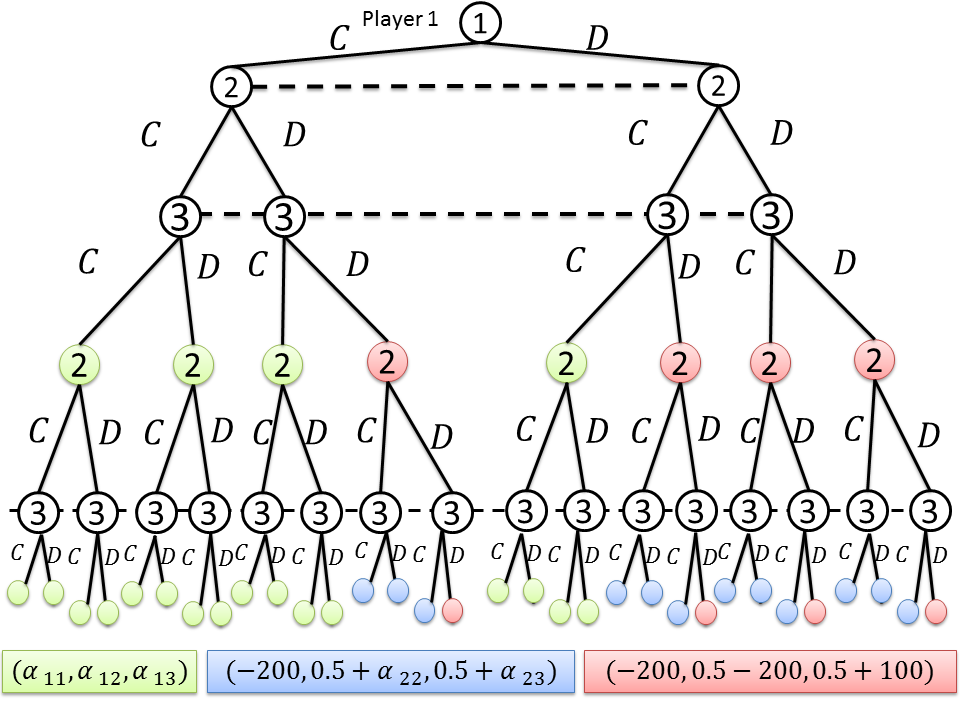
\includegraphics[scale=0.28]{Figures/1.5qubit/FigurasRevistas/Slide1.png}
\caption{Extensive form representation of the classic Pirate Game for $3$ players. }
\label{fig:pg_architecturegametree:extensiveform}
\end{figure}

The green accent, in Figure \ref{fig:pg_architecturegametree:extensiveform}, shown in the nodes represent a state where the first captain (player $1$), will see her proposal accepted, the utility associated . The blue accent denotes the outcomes where the second captain makes a proposal and has seen it accepted. The red accent color represents the outcomes where the player $3$ will be the remaining pirate.

The number of coins will translate directly the utility associated receiving them. The highest ranking pirate in the hierarchy is responsible to make a proposal to divide the 100 gold coins. A captain $i$ chooses the amount of coins a player $j$ get; this amount will be represented by $\alpha_{ij}$. In the initial stage of the game the captain will define $\alpha_{11}, \alpha_{12}, \alpha_{13}$, according to Equation \ref{eq:goodss} ($N$ the number of pirates in the game). 

\begin{equation}
\label{eq:goodss}
\forall i \in \{1 , 2, ..., N-1\} : \sum_{j=i}^{N}\alpha_{ij}=100, \forall i,j :\alpha_{ij}\in\mathbb{N}_{0}
\end{equation}

The values for $(\alpha_{11}, \alpha_{12}, \alpha_{13})=(99, 0, 1)$ will be the allocation that results in an equilibrium for the $3$ player game .

If the proposal is rejected the captain will be thrown off board, and the captain he will receive a negative payoff of $-200$. The pirates have also an incentive to climb the hierarchy; accounted by adding an expected value of half a coin ($0.5$), to the payoff of the remaining players if the voting fails. This tie breaker and death penalty is shown in Figure \ref{fig:pg_architecturegametree:extensiveform}.

\section{Quantum Model}
\subsubsection{Game system: Setting up the Initial State}
\label{subsec:pirates_initialstate}

A game $\Gamma$ can be viewed as a system composed by qubits manipulated by players. We will use the definition of quantum game discussed in Section \ref{sec:background_quantum_game_theory}, to model our game system. Akin to the Quantum Ultimatum game desbribed in \cite{Fra2011}, our objective is to apply that quantization scheme to the normal form representation of the game tree in Figure \ref{fig:pg_architecturegametree:extensiveform}.


In this $3$ player game there will be $5$ qubits representing the actions or the players decision; three qubits will represent the first voting round, the other two will portray the actions of the second voting round.
The number of qubits needed to represent the game grows exponentially with the number of players. For $N$ players we need $\sum_{i=2}^{N}{i}$ qubits. With 8 players, this game would already be impractical to simulate in a classical computer. In this regard a quantum computer may enhance our power to simulate this kinds of experiments \cite{Rieffel2011}.

The mapping function $\xi$ that assigns each action/qubit $\varphi_{j}$ ( with $j=\{ 1, 2, 3, 4, 5\}$), to a player is represented on Equation \ref{playerxiximapping}. 

\begin{equation}
\xi(j)=\begin{cases}
1 & ,\; if\; j=1;\\
2 & ,\; if\; j\in\{2,4\};\\
3 & ,\; if\; j\in\{3,5\}.
\end{cases}
\label{playerxiximapping}
\end{equation}

With $3$ players and $5$ actions our system with be represented in a $\mathcal{H}^{32}$ using a state $\psi$. This means that to represent our system we will need $2^{5}\times 1$ vectors, our system grows exponentially with the number of players/qubits. Each pure basis  of $\mathcal{H}^{32}$ will represent a possible outcome in the game. We assign a pure basis as $\vert 0\rangle = \vert C\rangle$ (``C'' from ``Cooperate''), and $\vert 1\rangle = \vert D\rangle$ (``D'' from ``Defect''). 




The initial system ($\vert \psi_{0}(\gamma) \rangle$), will be set up by defining an entanglement coefficient $\gamma$, that affect the way the five qubits (belonging to the three pirate players), are related; this is shown in Equation \ref{eq:estado_inicial_pg}. 
We will entangle our state by applying the gate $\mathcal{J}$ \cite{Letters2002}. The parameter $\gamma$ becomes a way to measure the entanglement in the system\cite{Eisert2008}. 

We analysed the role of the entanglement of the system since other examples researched pointed to it being the prominent factor regarding behaviour changes from the classsical perspective\cite{Fra2011a}\cite{Fra2011}\cite{Letters2002}\cite{Khan2011}\cite{Ricketts2006}. 


\begin{equation}
D=\left[\begin{array}{cc}
0 & 1\\
1 & 0
\end{array}\right]
\label{eq:DDDDDDDrica}
\end{equation} 



\begin{equation}
\mathcal{J}=exp\left\{ i\frac{\gamma}{2} D \otimes D \otimes D \otimes D 
\otimes D
\right\} 
\label{eq:matrix_exponencial_esoterica}
\end{equation} 

\begin{center}
\begin{equation}
%\vert \psi_{0}(\gamma) \rangle= cos( \frac{\gamma}{2})\vert 00\rangle+ isin(\frac{\gamma}{2})\vert 11 \rangle, \gamma \in (0,\pi)
\begin{split}
\vert\psi_{ini}(\gamma)\rangle=exp\left\{ i\frac{\gamma}{2} D \otimes D \otimes D \otimes D 
\otimes D\right\} \vert00000\rangle \\
=cos(\frac{\gamma}{2})\vert00000\rangle+isin(\frac{\gamma}{2})\vert11111\rangle,\gamma\in(0,\frac{\pi}{2})
 \end{split}
\label{eq:estado_inicial_pg}
\end{equation}
\end{center}



\subsubsection{Strategic Space}
\label{subsec:strategic_space}

The strategic space is a set of unitary operators that the players can use to manipulate their assigned qubits.

Each player will have a strategy $\tau_{i}$  which assigns a
unitary operator $U_{j}$ to every qubit $j$ that is manipulated
by the player ($j$$\in\xi^{-1}(i)$). $\tau_{2}= \{D_{2},C_{4}\}$ represents the strategy where the player $2$ votes $D$ in the first stage and $C$ in the second stage.

\begin{equation}
\begin{split}
\varphi_{j} = a . \vert C \rangle + b . \vert D \rangle , \\  j \in \{ 1, 2, 3, 4, 5 \}, \\ \{ a,b \} \in \mathbb{C} : a^2 + b^2 =1
\end{split}
\label{eq:opvarphiquantumstates}
\end{equation}

Each player will be able to manipulate her assigned qubits $j$ with an unitary operator of the form shown in Equation \ref{eq:general_unitary_special_one} (shown in Section \ref{sec:background_quantum_game_theory} $\mathcal{U}_{j}(w,x,y,z)=w.I + ix.\sigma_{x} + iy.\sigma_{y} + iz.\sigma_{z}, $ with $ w,x,y,z \in \mathbb{R} \wedge  
w^2 + x^2 + y^2 + z^2 =1 $). However in  order to explore the potential of quantum strategies, \cite{Eisert2008} proposes that it is sufficient to restrict the strategic space span by to the $2$-parameter (polar coordinates), set of matrices in Equation \ref{eq:operadoresinfinitus}, with $ \theta \in ( 0, \pi )$, and $\phi \in ( 0, \frac{\pi}{2})$. We will try to use the strategic space $\mathcal{U}_{j}(\theta,\phi)$ to represent our player's actions.



\begin{equation}
\begin{split}
\mathcal{U}_{j}(\theta,\phi) = \left[\begin{array}{cc}
cos(\frac{\phi}{2}) & e^{i\phi}sin(\frac{\phi}{2})\\
-e^{-i\phi}sin(\frac{\phi}{2}) & cos(\frac{\phi}{2})
\end{array}\right] , \\  j \in \{ 1, 2, 3, 4, 5 \}, \theta \in ( 0, \pi ) , \phi \in ( 0, \frac{\pi}{2})
\end{split}
\label{eq:operadoresinfinitus}
\end{equation}


 However the two operators that correspond to the original classical actions of voting ``Yes'' or to Cooperate, and voting ``No'' (Defect) are not entirely characterized by the subset $\mathcal{U}_{j}(\theta, \phi)$. These classical actions belong to a subset $S_{j}$ described in Equation \ref{eq:operators_piratas_quanticos}.  
The classical cooperation operator will be represented by the Identity operator ($o_{j0}$, where $j$ identifies the qubit that the respective player will act upon). When assigned to a qubit this operator will leave it unchanged. This operator is described by Equation \ref{eq:operadoresinfinitus} when $\mathcal{U}(0,0)$.

The defection operator ($D$), is represented by one of Pauli's Operators - the Bit-flip operator. This operator was chosen because it performs the classical operation NOT on a qubit. 
Within the restricted space $\mathcal{U}_{j}$, approximate alternative for the defect operator in the set $\mathcal{U}_{j}$ is $\mathcal{U}_{j}(\pi, 0)$; they are interchangeable when $\gamma = 0$. For $\gamma >0$ we will include the pure strategy $D$ represented by the Bit-flip operator into our restricted strategic scape $\mathcal{U}_{j}$.



\begin{equation}
S_{j} = \begin{cases}
C_{j} = o_{j0}=\left[\begin{array}{cc}
1 & 0\\
0 & 1
\end{array}\right]\\
D_{j} = o_{j1}=\left[\begin{array}{cc}
0 & 1\\
1 & 0
\end{array}\right]
\end{cases} , j \in \{ 1, 2, 3, 4, 5 \}
\label{eq:operators_piratas_quanticos}
\end{equation}






The notation for the pure basis as $\vert C\rangle$ refers to a quantum state and should not be confused as a Cooperate operator $C$ that is a matrix (the identity matrix). A original player quantum state (the qubits of the form $\varphi_{j}$) is defined by Equation \ref{eq:opvarphiquantumstates}.





\subsubsection{Final State}
\label{subsec:pirates_finalstate}


This final state is calculated by constructing a super-operator, by performing the tensor product of each player chosen strategy, from Equation \ref{eq:operadoresinfinitus} or \ref{eq:operators_piratas_quanticos}. The super-operator, containing each player's strategy, will then be applied to the initial state,as shown in Equation\ref{eq:piratas_final_move}.

\begin{equation}
\vert\psi_{fin}\rangle=\otimes_{i=1}^{3}\otimes_{j\in\xi^{-1}(i)}\mathcal{U}_{j}\vert\psi_{ini}(\gamma)\rangle
\label{eq:piratas_final_move}
\end{equation}


In order to calculate the expected payoff functions we need to de-entangle the system, before measuring. The act of measuring, in quantum computing, gives an expected value that can be understood as the probability of the system collapsing into that state. In the Figure \ref{fig:pg_architecture3players} we have represented the way we entangle and de-entangle the system.

\begin{figure}[h]
\centering 
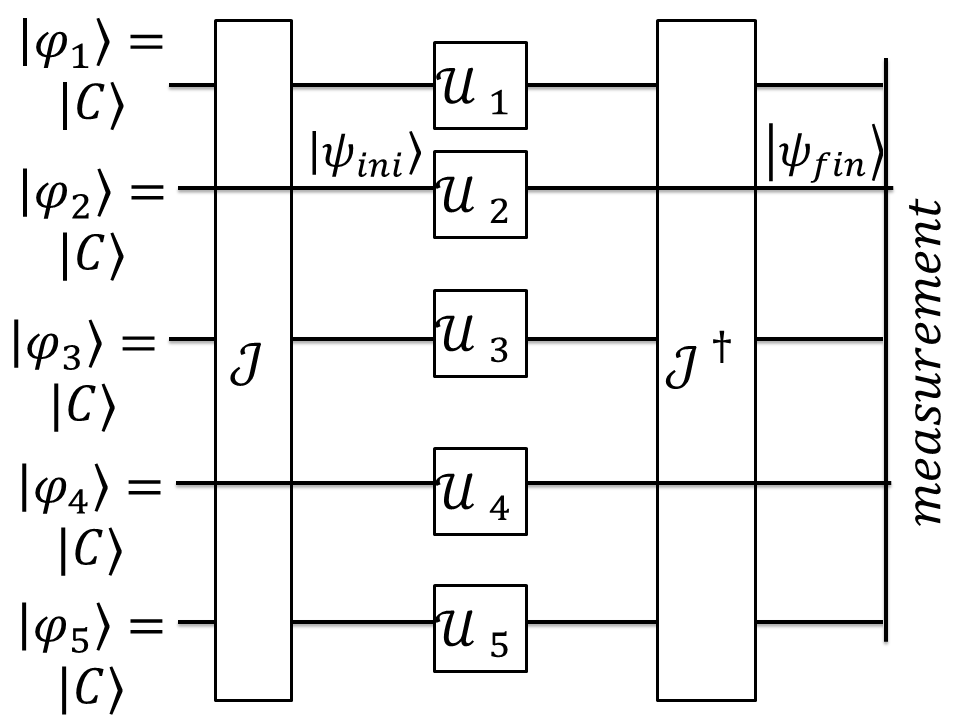
\includegraphics[scale=0.14]{Figures/architecture/esquema/esquema.png}
\caption{Scheme that represents the set-up of the $3$-player Pirate Game. Before we measure the final result we need to apply the transpose operator $\mathcal{J}^{\dagger}$. }
\label{fig:pg_architecture3players}
\end{figure}






\subsubsection{Utility}
\label{subsec:pirates_utility}

To build the expected payoff functionals for the three player situation we must take into account the sub-games created when the proposal is rejected, in Figure \ref{fig:pg_architecturegametree:extensiveform}.


These utility functions will represent the degree of satisfaction for each pirate after game by attributing a real number to a measurement performed to the system.


We can observe in Figure \ref{fig:pg_architecturegametree:extensiveform} that in that we have three separate groups (denoted by the colour accents), of outcomes that share the same payoff, in the original problem. 
In our quantum scheme we can aggregate the pure-basis quantum states ($\mathcal{B}$), associates with a payoff in the following manner: 
\begin{itemize}
\item States where the first proposal is accepted - ``Accepted 1' (or $A_{1}$), with a green colour accent in Figure \ref{fig:pg_architecturegametree:extensiveform}. If ($P(A_{1})=1$) the players can expect to receive the following payoff: $(a_{11}, a_{12}, a_{13})$.

\item States where the first captain will be eliminated and the second player gets her proposal accepted  - ``Accepted 2'' (or $A_{2}$) with a blue colour accent in Figure \ref{fig:pg_architecturegametree:extensiveform}. If $P(A_{2})=1$, then the expected payoff is $(-200, a_{22}+0.5, a_{23}+0.5)$.

\item States where all proposals are rejected  - ``Rejected 2' (or $R_{2}$)' with a red colour accent in Figure \ref{fig:pg_architecturegametree:extensiveform}. If both proposals are rejected ($P(R_{2})= 1$), the players might expect to receive $(-200, -200+0.5, 100+0.5)$.

\end{itemize}

In order to calculate the probability of the final state collapsing onto a basis state $b \in \mathcal{B}$ we perform a projection of the state in the chosen basis and we measure the squared length of the projection, $P(b) = \vert\langle b\vert\psi_{fin}\rangle\vert^{2}$\cite{Trueblood}. The expected utility function for each player will be a weighted average of all possible outcomes. The expected utility for player $1$, shown in Equation \ref{eq:pirates_payoff32:1}, give a real number that represents the payoff associated with a final state. The same goes to player $2$ that has her expected utility functional specified in Equation \ref{eq:pirates_payoff32:2}, and the player $3$ in Equation \ref{eq:pirates_payoff32:3}.


\begin{equation}
\begin{split}
P(A_{1}) = \sum_{x_{3}}\sum_{x_{4}}\vert\langle0,0,0,x_{4},x{5}\vert\psi_{fin}\rangle\vert^{2} + \\  + \sum_{x_{3}}\sum_{x_{4}}\vert\langle1,0,0,x_{4},x{5}\vert\psi_{fin}\rangle\vert^{2} + \\ 
+ \sum_{x_{3}}\sum_{x_{4}}\vert\langle0,1,0,x_{4},x{5}\vert\psi_{fin}\rangle\vert^{2} + \\ 
+ \sum_{x_{3}}\sum_{x_{4}}\vert\langle0,0,1,x_{4},x{5}\vert\psi_{fin}\rangle\vert^{2}
\end{split}
\end{equation}

\begin{equation}
\begin{split}
P(A_{2}) = \sum_{x_{5}}\vert\langle1,1,1,0,x{5}\vert\psi_{fin}\rangle\vert^{2} + \vert\langle1,1,1,1,0\vert\psi_{fin}\rangle\vert^{2} + \\ + \sum_{x_{5}}\vert\langle1,1,0,0,x{5}\vert\psi_{fin}\rangle\vert^{2}+ \vert\langle1,1,0,1,0\vert\psi_{fin}\rangle\vert^{2} + \\ 
+ \sum_{x_{5}}\vert\langle1,0,1,0,x{5}\vert\psi_{fin}\rangle\vert^{2} + \vert\langle1,0,1,1,0\vert\psi_{fin}\rangle\vert^{2}
+ \\ + \sum_{x_{5}}\vert\langle0,1,1,0,x{5}\vert\psi_{fin}\rangle\vert^{2} + \vert\langle0,1,1,1,0\vert\psi_{fin}\rangle\vert^{2}
\end{split}
\end{equation}

\begin{equation}
\begin{split}
P(R_{2}) = \vert\langle1,1,1,1,1\vert\psi_{fin}\rangle\vert^{2} + \vert\langle1,1,0,1,1\vert\psi_{fin}\rangle\vert^{2} + \\ 
+ \vert\langle1,0,1,1,1\vert\psi_{fin}\rangle\vert^{2}
+ \vert\langle0,1,1,1,1\vert\psi_{fin}\rangle\vert^{2}
 \end{split}
\end{equation}


   

 
\begin{equation}
\begin{split}
E_{1}(\vert\psi_{fin}\rangle)=\alpha_{11}\times P(A_{1}) - \\ 
 - 200\times( P(A_{2})  +  P(R_{2}) ) 
 ) 
\end{split}
\label{eq:pirates_payoff32:1}
\end{equation}

\begin{equation}
\begin{split}
E_{2}(\vert\psi_{fin}\rangle)=\alpha_{12}\times P(A_{1}) - \\
 + (0.5 + \alpha_{22})\times P(A_{2})  + \\ 
+(0.5-200)\times P(R_{2})
\end{split}
\label{eq:pirates_payoff32:2}
\end{equation}

\begin{equation}
\begin{split}
E_{3}(\vert\psi_{fin}\rangle)=\alpha_{13}\times P(A_{1}) + \\
 + (0.5 + \alpha_{23})\times P(A_{2})   + \\
 + (100.5)\times P(R_{2}) 
\end{split}
\label{eq:pirates_payoff32:3}
\end{equation}



The gate $\mathcal{J}$ is chosen to be commutative with the super-operators created by the tensor product of the classical actions $C$ (cooperate, indicated by the identity matrix and $\mathcal{U}(0,0)$)), and $D$ (defect, indicated by the Bit-flip operator matrix, and $\mathcal{U}(\pi,0)$ when $\gamma = 0$)). For example $[ \mathcal{J} , C \otimes D \otimes C \otimes C \otimes D ] = 0 $.


This condition implies that choosing any operator from the sub-set $O = \{ \mathcal{U} ( \theta , 0) , \theta \in (0, \pi) \}$ with $\gamma = 0$ is the equivalent of a classical mixed action. A strategy $\tau_{i}$ is a classical pure strategy iff all operators in the strategy belong to the subset $S$ (defined in \ref{eq:operators_piratas_quanticos}). A strategy $\tau_{i}$ is a classical mixed strategy iff all operators in the strategy belong to $O$.
If the parameter $\phi$ in the operator $U_{j}(\theta ,\phi)$ differs from $0$, and the entanglement parameter $\gamma = 0$ we are able to explore quantum strategies that have no counterpart in the classical domain\cite{Eisert2008}.









\section{Analysis and Results}
\label{sec:pirate_results}
We tried to get our Quantum Model of the Pirate Game as close as possible in order to compare the the original game. However we did not incorporate the concept of measuring the results between rounds of voting. In the original problem after each stage the results are accounted. Our approach was deemed more adequate to analyse in \cite{Fra2011}.

In works such as the Prisoner's Dilemma\cite{Letters2002}\cite{Eisert2008}, and Quantum Ultimatum Game\cite{Fra2011}, the strategic space was analysed allowing a infinity of mixed quantum strategies. Our game space was much more vast than the works previously mencioned, we used $5$ qubits to model our system, their models had no more than $3$ qubits. This imposed that in order to analyse our system while conceptualy, our strategic space is also infinite, we restricted in order to analyse. In particular we payed special interest in the strategies: $C$, $D$, $\mathcal{U}(\pi, 0)$, and $\mathcal{U}(0, \frac{\pi}{2})$. The first two mensioned strategies are the equivalent of the classical strategies ``Cooperate'' and ``Defect'', the other two are quantum strategies. Toghether these $4$ strategies when paired with the coefitients $(w,x,y,z)$ are known to span a class that contains all unitary operators, the $\mathsf{SU}(2)$. According to \cite{Du} these $4$ operators when the entanglement is maximum provided a cycle where each operator was an optimal counter strategy to other. 

The set-up of the initial system was crucial to introduce the phenomenon of entanglement. We concluded that without entanglement the game has a strictly determined solution and behaves as the original problem, however there are more pure strategy Nash Equilibria.

For the $2$-player game we concluded that the expected utility when the players use a mixed strategy Nash equilibrium renders an expected utility of $(25, 25.125)$ wich is also a Pareto optimal solution because it is not possible to improve one player's expected utility without harm the other. The classical setting is more beneficial to the captain in this game, because she will receive the 100 coins. We also found that distributing 50 coins would give a lower expected utility to the captain. This result is interesting because it is a Pareto optimal solution in the classical version, though not a Nash Equilibrium, and it renders an higher payoff than the Nash Equilibrium and Pareto Optimal solution when the sytem is maximaly entangled and the players have access to the $4$ pure quantum strategies discussed in \cite{Du} and \cite{Letters2002}. 

The $3$-player game also has a mixed quantum strategy Nash Equilibrium, like the $2$-player game, when the entanglement is maximum, however its calculus fell beyond the scope of this dissertation. 

When trying to find if it is possible for the captain in the first stage of the game to acquire all gold coins we found that if the other players have a restricted set of strategies, they can only use the classical Cooperate or Defect operators, and if they don't know that the captain has access to quantum strategies, the captain will be able to get the $100$ gold coins. However if players $2$ and $3$ have a restricted set where they can only use the classical Cooperation operator, or the classical Defection operator, the player $1$ will no longer be able to acquire the 100 coins with certainty. Instead she may be able to acquire the $100$ coins with probability $\frac{1}{2}$ or end up thrown off board with equal probability.

These results corroborate the literature in the Chapter 3, while contributing with another case study.

\section{Conclusion}

With this dissertation we developed an approach to a novel Quantum Game - the Pirate Game. While defining the quantum model of the game we found that the most unique features of the problem, that appear when the number of coins does not allow for the captain to bribe the necessary votes in order for him to be spared, would pose an hard problem to analyse because of the exponential growth the system experiences when we increase the number of qubits. Possibly with the advent of the first commercial quantum computers these we will have resources to simulate these kinds of systems in a more spacial optimized way - the physical model for a qubit can be the polarization of a photon. 

Nevertheless we developed a model for the Quantum Pirate Game with $3$ players, and we also studied the system for $2$ players. Both games are strictly determined in the original problem, however when we allow the system to be entanglement we start noticing that  there are quantum operators that can cause interference. When the game is maximally entangled, we could not find a pure strategy Nash Equilibrium. These results are similar to the findings in models such as the Prisoner's Dilemma\cite{Eisert2008}\cite{Letters2002}, and Stackelberg Duopoly \cite{Khan2011}.

We also found that, when the system is maximally entangled, if we restrict the strategic space for some players we break the cycle of optimal quantum counter-strategies suggested by \cite{Du}: when the entanglement is maximal, $\mathcal{U}(\pi, 0)$ is the optimal counter-strategy for $C$ (represented by the identity marix), $\mathcal{U}(0, \frac{\pi}{2})$ is the optimal counter strategy for $\mathcal{U}(\pi, 0)$, $D$ becomes the optimal counter-strategy for $\mathcal{U}(0, \frac{\pi}{2})$, and $C$ becomes an optimal counter strategy for $D$. This means that it is possible for a player to explore this weakness if other players are unaware. If we had a quantum gambling system, or a voting system such as in the Pirate Game, the strategic space and the entanglement are information that needs to be available for all players equally in order for them to choose their best-response.

Another contribution from this thesis is the simulation code in Matlab provided in the appendices, these examples might be used in order to experiment the quantum models of the Prisoner's Dilemma, a Quantum Roullete, and finally the Quantum Pirate Game. We also developed a Matlab simulation of the Quantum agorithms Walk in a Line. These simulations were built while analysing related work on the area.

The implications of Quantum Mechanics are still very dettached from the way we think. The Quantum theory is deeply rooted in the concept of probability. Robert Laughlin uses the concept of emergence to explain the way classical phenomena arises from quantum mechanics\cite{Laughlin2005}. It is almost poetic that in our apparently deterministic world arises with all its patterns surges from the chaos. 

\subsection{Future Work}
The principles of quantum computing provide an extremely rich source of ideas to extend other fields of knowledge.
Some suggestions for possible extensions for this work would be:

\begin{enumerate}


\item \textbf{Optimize this Quantum Pirate Game Model.} To model this game as a Quantum Bayesian Network. 

\item \textbf{To implement and test this quantum model with human subjects.} The field of Quantum Cognition tries to explain the Human reasoning process by using principles from quantum game theory, namely quantum probabilities. To expose subjects to a quantum model and having them try to take advantage of the rules of the system might provide valuable insights to the way we reason. 

\item \textbf{Increase the number of players.} Studying the quantum system with $8$ players and $1$ gold coin, would be an interesting extensions for this work. This would allow to experiment the bizarre survival situations that happens when there are not enough coins for the captain to bribe the other pirates. However this particular case of the pirate game would need a $35$-qubit system in order to be studied ($8$ qubits for the first stage, $7$ for the second stage, until reaching a $2$-player sub-game). In a classical computer and full joint probability this would mean working with vectors in the scale $10^{10}$.

\item \textbf{A graphical user interface (GUI) for the Pirate Game.} This would provide a more approachable way to tweak parameters.

\item \textbf{To create and structure a platform to promote scientific dissemination of quantum computing.} While investigating and developing this solution, there was often the thought that it would be important for undergraduate Computer Science students to come with contact with this paradigm. This field is still shrouded with mystery to many people, and this makes it a priority topic for scientific divulgation. 
\end{enumerate}

 
 






%\bibliographystyle{IEEEtran}
%\bibliographystyle{splncs}
%\bibliographystyle{ieeetr}
%\bibliography{02.biblio}

\bibliographystyle{IEEEtran}
\bibliography{02.biblio}



\end{document}
